\documentclass[10pt]{article}
\usepackage{icmlko}

\icmlmeta{IP 파운데이션 월드모델}{283}{빌려온 도메인}{시장 레코드 207건에 쓸 신호가 있다 --- 그런데 팝업에 붙이면 마스크 무늬가 출처 표지가 된다}

\begin{document}

\twocolumn[
\icmlheader

\begin{abstract}
노트 282가 ``문이 열렸는데 들어갈 것이 없다''로 끝났다. 팝업은 75행(학습
16 · 유보 59)이라 청력 문턱 22 아래이고 판 몫이 2.3\% 이며, 레코드에서 뽑을
수 있는 전용 축은 노트 276$\sim$277이 다 털었다. \textbf{들어갈 것을 밖에서
찾았다} --- 하네스 트랙이 크롤링해 둔 \textbf{시장 레코드 647건}이다. 방문
라벨 $+$ 단일 이벤트가 \textbf{207건}으로 팝업의 2.8배다. 신호가 있나 먼저
쟀다. 첫 수는 \textbf{기간 일수 $+$0.535} 로 제일 셌는데, 라벨이 \emph{총}
방문이라 그렇다 --- 이 실험실의 팝업 라벨은 \texttt{y\_perday} 이고 바로
그 교락을 빼려고 그렇게 정의돼 있다. 일평균으로 다시 재니 \textbf{$-$0.061}
로 사라진다(노트 133). \textbf{나머지는 살아남는다} --- 멀티스토어
$+$0.227 · IP 이력 $+$0.217 · 그리고 \textbf{\texttt{category} 가 제일
세다}(크루스칼 $H{=}29.4$, $p{=}0.0001$; game\_webtoon 3,979/일 대 fashion
810/일). \texttt{category} 는 지금 팝업에 \textbf{없는} 축이다. 그런데 붙일
수가 없다. 두 라벨이 같은 log10 자인데 \textbf{시장이 통째로 0.46 위}(3.2배)
이고, 사분위마다 거의 일정하다. 계수 방식 차이는 아니다 --- 같은 이벤트를
직접 잰 둘이 $\times$1.19 · $\times$1.07 이었다. \textbf{기사가 되는 팝업이
원래 큰 것}이다. 그래서 붙이면 이렇게 된다: 내부 75행은 손 축 마스크가
\textbf{100\%}, 시장 207행은 \textbf{0\%} --- \textbf{마스크 무늬가 곧 출처
표지이고 출처가 라벨을 3.2배로 가른다.} 노트 266의 ``기록됐나'' 덫과 같은
자리다. \textbf{결론: 붙이지 말고 도메인을 새로 연다.} 학습 101행(청력 문턱
22 위) · 유보 106행 · 판 몫 4.0\%.
\end{abstract}
]

\section{들어갈 것을 밖에서 찾는다}

노트 276$\sim$282가 팝업의 전용 축을 다 털었다. 후보 열여섯 $\to$ 넷 $\to$
전부 무용($-$0.0070). 노트 282의 마지막 줄이 \textbf{``문보다 들어갈 것이
없는 게 문제다''} 였다.

그런데 이 저장소에는 lab 이 한 번도 안 쓴 층이 있다. 하네스 트랙이 크롤링해
둔 \textbf{시장 레코드 647건}이다.

\begin{center}\small
\begin{tabular}{lr}
\hline
시장 레코드 & 647 \\
방문 라벨 있음 & 328 \\
단일 이벤트(집계형 제외) & 309 \\
\textbf{둘 다} & \textbf{207} \\
\hline
지금 lab 의 팝업 & 75 \\
\hline
\end{tabular}
\end{center}

\section{첫 수가 교락이었다}

\begin{figure*}[t]
\centering
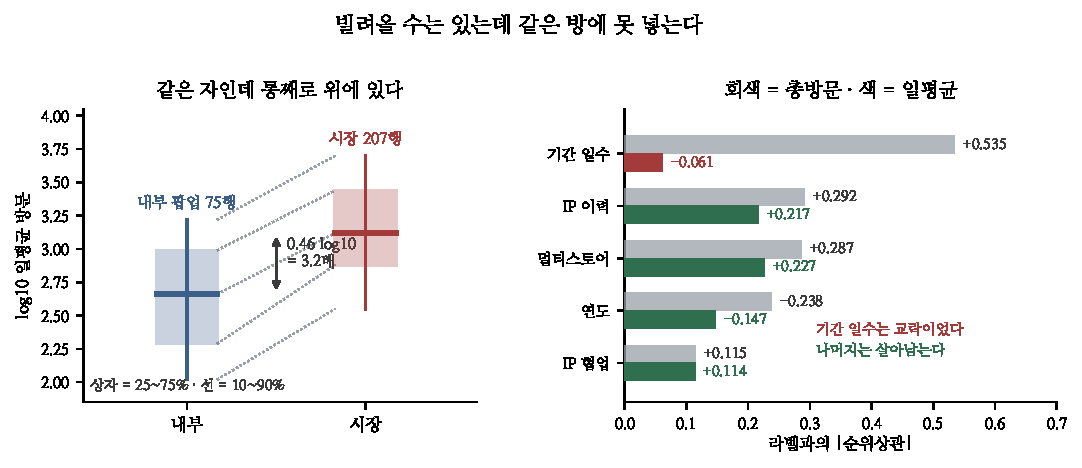
\includegraphics[width=\textwidth]{figs/borrow.pdf}
\caption{왼쪽 --- 두 라벨 분포. 상자가 25$\sim$75\%, 선이 10$\sim$90\%.
오른쪽 --- 필드별 라벨 상관. 회색이 총방문 기준, 색이 일평균 기준.}
\end{figure*}

가진 필드로 제 라벨의 순위를 매길 수 있나 물었다. 제일 센 것이 \textbf{기간
일수 $+$0.535} 였다.

\textbf{그대로 채택하면 안 된다}(노트 133). 저 라벨은 \emph{총} 방문이고,
오래 하면 총합이 크다. 이 실험실의 팝업 라벨이 \texttt{y\_perday} 인 것이
바로 그래서다 --- 그리고 노트 276이 \texttt{기간\_일수}를 팝업 축에서 뺀
이유도 같다(\texttt{y\_perday} 의 \textbf{분모}였다).

같은 눈금(일평균)으로 다시 쟀다.

\begin{center}\small
\begin{tabular}{lrr}
\hline
필드 & 총방문과 & 일평균과 \\
\hline
\textbf{기간 일수} & $+$0.535 & \textbf{$-$0.061} \\
멀티스토어 & $+$0.287 & $+$0.227 \\
IP 이력 & $+$0.292 & $+$0.217 \\
연도 & $-$0.238 & $-$0.147 \\
IP 협업 & $+$0.115 & $+$0.114 \\
\hline
\end{tabular}
\end{center}

\textbf{제일 세던 것만 사라지고 나머지는 그대로다.} 그리고 집단 축은
\emph{오히려 세진다}.

\begin{center}\small
\begin{tabular}{lrr}
\hline
& 총방문 & 일평균 \\
\hline
\texttt{category} & $H{=}23.6$ & \textbf{$H{=}29.4$} ($p{=}0.0001$) \\
\texttt{venue\_type} & $H{=}5.4$ & $H{=}5.3$ ($p{=}0.15$) \\
\hline
\end{tabular}
\end{center}

\texttt{category} 의 폭이 다섯 배다 --- game\_webtoon 3,979/일 ·
character 1,925 · beauty 1,800 · fnb 1,250 · other 1,250 ·
entertainment 1,000 · \textbf{fashion 810}. \textbf{그리고 이건 지금 팝업에
없는 축이다.} \texttt{venue\_type} 은 못 가르는데, 팝업이 이미
\texttt{venue\_prominence} 를 갖고 있으니 마침 잘 됐다.

\section{그런데 같은 방에 못 넣는다}

두 라벨을 나란히 놓으면 \textbf{같은 log10 자인데 시장이 통째로 위}다.

\begin{center}\small
\begin{tabular}{lrrrrr}
\hline
log10 일평균 & 10\% & 25\% & 50\% & 75\% & 90\% \\
\hline
내부 팝업 75행 & 2.02 & 2.29 & 2.66 & 2.99 & 3.22 \\
시장 207행 & 2.55 & 2.88 & 3.12 & 3.44 & 3.70 \\
\hline
차 & .53 & .59 & .46 & .45 & .48 \\
\hline
\end{tabular}
\end{center}

\textbf{사분위마다 거의 일정한 0.46$\sim$0.59, 즉 3.2배다.}

\paragraph{계수 방식이 아니다} 같은 이벤트를 내부 실측과 시장 주장으로 둘 다
가진 사례가 둘 있고 $\times$1.19 · $\times$1.07 이었다. \textbf{계수 부풀림은
$\times$1.1 수준이다.} 그러니 3.2배는 \textbf{선택}이다 --- 기사가 되는
팝업이 원래 크다. \textbf{라벨이 틀린 게 아니라 모집단이 다르다.}

\paragraph{그래서 덫이 된다} 순위 목표에서 일정 배수는 단조 변환이라 순위를
안 바꾼다. 그러니 언뜻 붙여도 될 것 같다. \textbf{안 된다.}

\begin{center}\small
\begin{tabular}{lrr}
\hline
& 내부 75행 & 시장 207행 \\
\hline
손 축 다섯 마스크 & \textbf{100\%} & \textbf{0\%} \\
라벨 중앙 & 2.66 & 3.12 \\
\hline
\end{tabular}
\end{center}

붙이면 \textbf{마스크 무늬가 곧 출처 표지}가 되고, 출처가 라벨을 3.2배로
가른다. 모형은 축을 안 보고 \emph{``손 축이 있나''} 하나로 순위를 맞출 수
있다. \textbf{노트 266의 덫과 같은 자리다} --- 그때는 토큰 없는 행이
설계행렬에서 전부 0 이라 ``기록됐나'' 방향이 생겼고, 그 축이 채택 검사
셋을 다 통과했었다.

\section{도메인을 새로 연다}

붙이는 대신 \textbf{열째 채점 도메인}으로 세운다. 마스크 무늬가 도메인
안에서 균일해지므로 덫이 사라진다.

\begin{center}\small
\begin{tabular}{lr}
\hline
학습행(2025년 이전) & \textbf{101} \\
유보행(2025년 이후) & \textbf{106} \\
판 몫(대략) & 4.0\% \\
\hline
청력 문턱(F18) & 22 --- \textbf{넘는다} \\
\hline
\end{tabular}
\end{center}

\textbf{학습 101행은 청력 문턱 22 위다} --- 이 도메인은 챔피언이 들을 수
있고, 전용 축(\texttt{category} 등)이 실제로 일할 수 있다. 팝업(16행)이 못
가진 조건이다.

\paragraph{먼저 확인할 것 셋} \textbf{①} 라벨 신뢰등급이 B 88 · C 82 ·
E 24 · D 11 · A 2 다 --- \textbf{C · D · E 가 117건(57\%)} 이고 노트 264의
정제 게이트를 이 도메인에도 걸어야 한다. \textbf{②} 시간 마스크 --- 시장
레코드의 \texttt{period\_from} 이 기사 날짜가 아니라 개최일인지 확인해야
한다. \textbf{③} 겹침 --- 내부 레코드와 같은 이벤트를 가리키는 시장 레코드가
있으면(메모리에 충전 후보 6건이 적혀 있다) 유보가 오염된다.

\paragraph{남은 것}
\begin{center}\small
\begin{tabular}{ll}
\hline
갈래 & 왜 \\
\hline
도메인 배선 & \texttt{state/audit.domains} 에 열째로 \\
라벨 정제 게이트 & C · D · E 57\% --- 하한값을 걸러야 \\
시간 마스크 확인 & \texttt{period\_from} 이 개최일인가 \\
내부와 겹침 & 같은 이벤트가 양쪽에 있으면 유보 오염 \\
\hline
\end{tabular}
\end{center}

\paragraph{규약} \textbf{두 자료를 붙일 때는 라벨 분포를 먼저 나란히 놓고,
마스크 무늬가 출처를 말하는지 본다.} 라벨이 같은 자를 쓰고 배수가 일정해도
--- 순위 목표라 배수는 무해해도 --- \textbf{결측 무늬가 출처를 말하면 그것이
곧 라벨을 말한다.} 노트 266에 이어 두 번째다.

\end{document}
